\documentclass[12pt,onecolumn,a4paper]{article}
\usepackage{epsfig,graphicx,subfigure,amsthm,amsmath}
\usepackage{color,xcolor}     
\usepackage{xepersian}
\settextfont[Scale=1]{sahel.ttf}
\setlatintextfont[Scale=1]{Times New Roman}
\graphicspath{ {./img/} }



\begin{document}


\title{گزیده و نکات بخش دوم، آماره‌های توصیفیِ نمونه‌ها\\\lr{"Introductory Statistics" by Wonnacott}} 
\author{مهدی صادق‌زاده قمصری}
\date{بهمن ۹۹}
\maketitle

\section{آماره} 
هدف اولیه علم آمار، بدست آوردن استنباطی درباره جامعه از طریق نمونه آن است. یک گام اولیه می‌تواند این باشد که نمونه را در چند عدد به طور خلاصه توصیف کرد. به هر کدام از این اعداد توصیف‌کننده‌ی نمونه، آماره\footnote{\lr{statistic}}ی نمونه گفته می‌شود.

\section{تکرار\footnote{\lr{frequency}}}
\begin{itemize}
    \item فضای گسسته \\
        متغیر تصادفی \lr{X} متغیر تصادفی گسسته نامیده می‌شود، اگر مقادیر آن محدود و یا نامحدود اما قابل شمارش باشند. خروجی انداختن تاس یک مثال از این متغیر هاست. برای ساده‌سازی درک نمونه، میتوان تکرار حالات مختلف نمونه را به عنوان یک آماره در نظر گرفت. آماره دیگر می‌تواند نسبت این تکرار ها به کل حالات\footnote{\lr{relative frequency}} باشد. \\
        در کنار هم قرار دادن این اعداد برای تمامی حالت یک متغیر تصادفی، به ما توزیع\footnote{\lr{distribution}} آنها را خواهد داد که با دیدن نمودار این توزیع‌ها یک تصور از نتیجه نمونه در ذهن شکل می‌گیرد. \\
        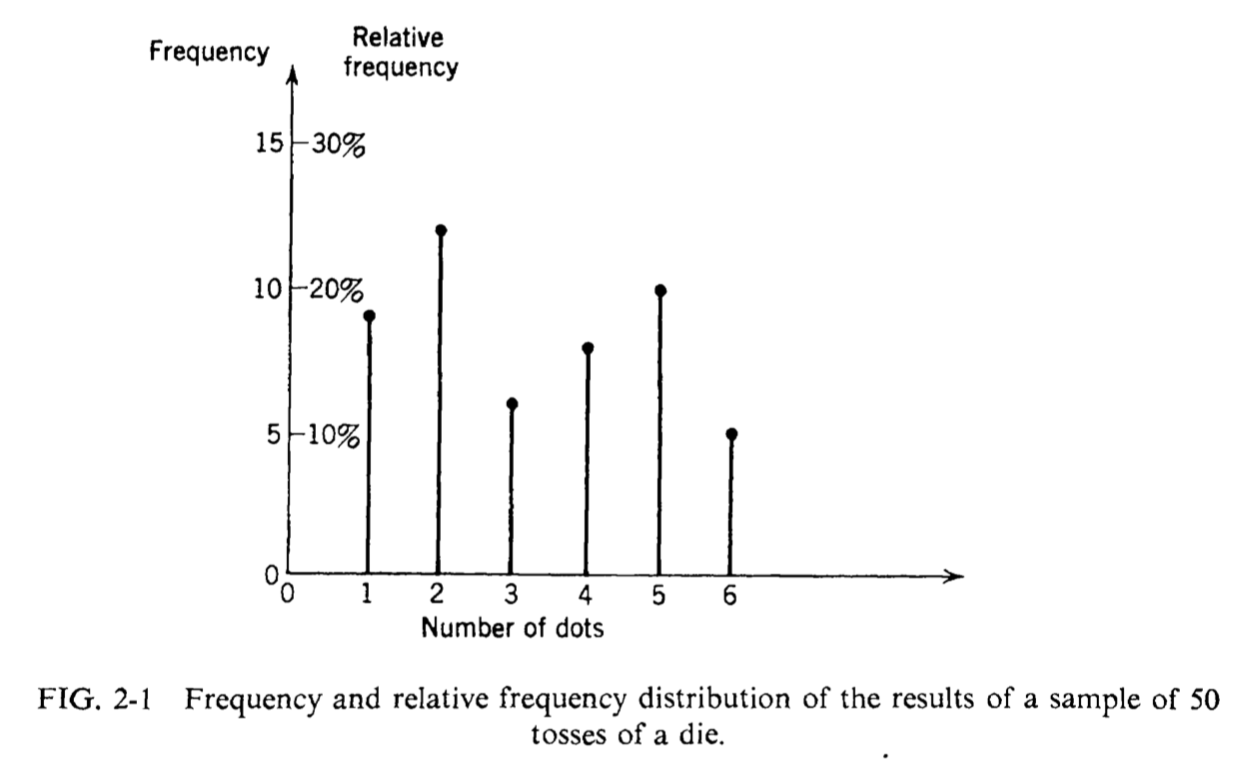
\includegraphics[width=\textwidth]{fig1.png}
    \item فضای پیوسته \\
        اگر نمونه متعلق به یک فضای پیوسته باشد، متغیر تصادفی \lr{X} می‌تواند هر مقداری بگیرد و دیگر تکرار یک مقدار مشخص از آن معنی ندارد(چون احتمال تکرار آن به صفر میل میکند)؛ نتیجتا به‌جای تکرار مقادیر مشخص، تکرار مقادیر در بازه های مشخص را می‌شمارند.\\
        تعداد این بازه ها باید با مجموعه حالات تناسب داشته باشد و همچنین وسط بازه ها، نمایانگر تمامی مقادیر بازه باشد.\\
        به نمودار توزیع این متغیر های تصادفی \lr{Histogram} نیز گفته می‌شود. \\
        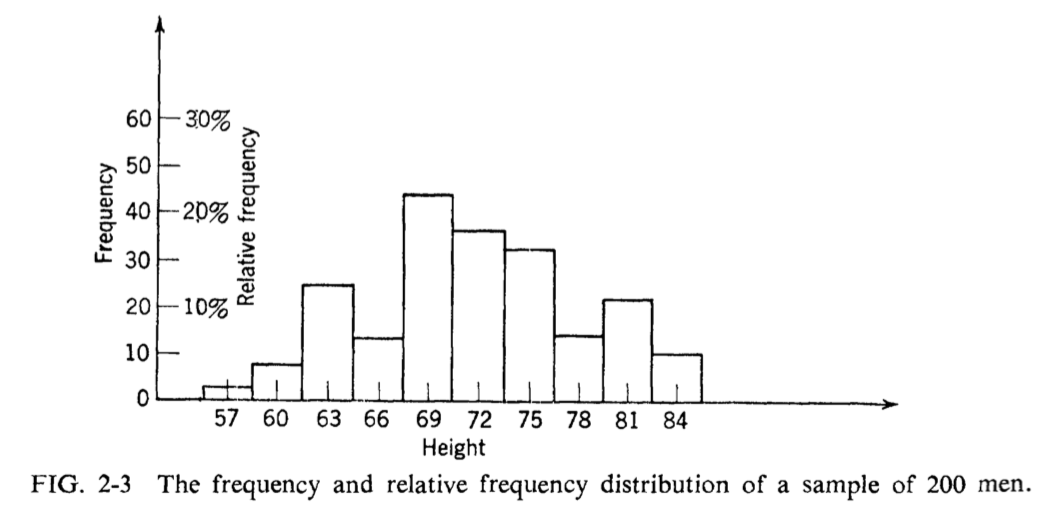
\includegraphics[width=\textwidth]{fig2.png}

\end{itemize}

برای توصیف توزیع تکرار یک نمونه، می‌توان از دو آماره توصیفی استفاده کرد: نقطه‌ی وسط توزیع و میزان گسترش توزیع.

\section{مقیاس های مکانی}
تعاریف مختلفی از "وسط" توزیع وجود دارد که ۳ تای از آنها مد، میانه و میانگین هستند.
\begin{itemize}
    \item مد\footnote{\lr{mode}}: بیشترین مقدار تکرارشده در نمونه \\
        این مقیاس مناسبی برای وسط یک نمونه نیست؛ زیرا به بازه‌بندی داده ها وابسته است؛ و همچنین می‌توان در یک توزیع چند نقطه بیشینه برابر داشت که این تعریف برای آنها گنگ بوده و به آن توزیع ها "bimodal" گفته می‌شود.
    \item میانه\footnote{\lr{median}}: پنجاه‌مین صدک داده‌ها \\
        بعضا به آن مقدار میانی نیز گفته می‌شود. اگر تنها داده از نمونه توزیع تکرار آن باشد، باید در انتخاب مقدار از بازه میانی دقت کرد.
    \item میانگین($\bar{X}$)\footnote{\lr{mean}}: حاصل تقسیم مجموع مقادیر نمونه بر تعداد آنها
        \begin{equation}
            \bar{X} \triangleq 1/n \sum_{i=1}^{n} X_i
        \end{equation}
        ییدر زمانی که با بازه ها سر و کار داریم؛ می‌توان مقادیر درون یک بازه را به طور تقریبی برابر مقدار وسط بازه درنظر گرفت:
        \begin{align*}
            \bar{X} \simeq 1/n(f_1 x_1 + f_2 x_2 + ... + f_k x_k) 
        \end{align*}
        نتیجتا:
        \begin{equation}
            \bar{X} \simeq \sum_{i=1}^{m} x_i(f_i/n)
        \end{equation}
\end{itemize}

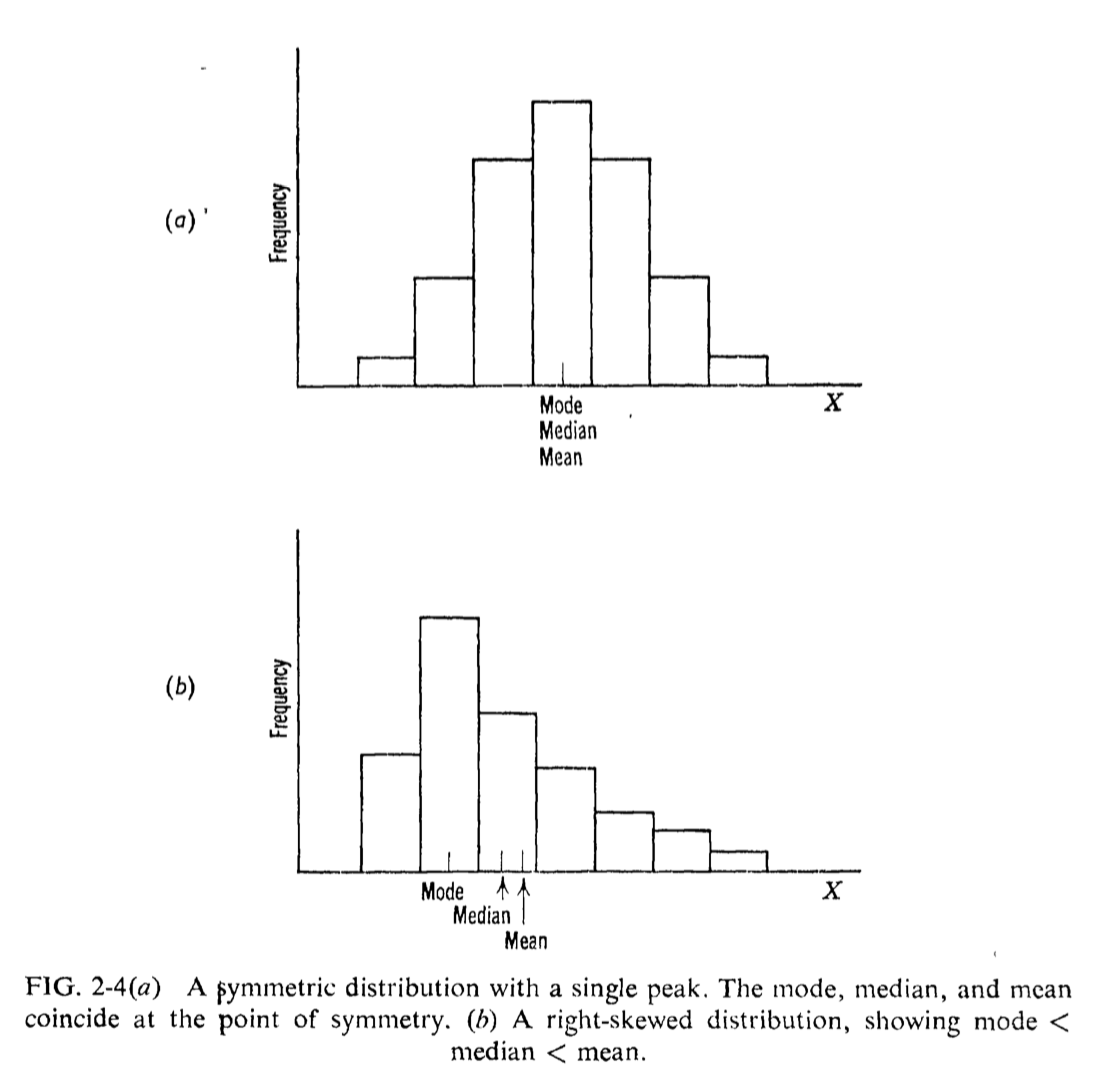
\includegraphics[width=\textwidth]{fig3.png}

نکات: \\
$\bullet$ برای تساوی ای که مبتنی بر تعریف است از نشانه \lr{$\overset{\Delta}{=}$} استفاده می‌کنیم. \\
$\bullet$ برای نشان دادن مقدار تقریبی از نشانه \lr{$\simeq$} استفاده می‌کنیم.


\section{مقیاس های پراکندگی}
ساده‌ترین مقیاس برای پراکندگی فاصله میان کوچک‌ترین و بزرگ‌ترین مقدار نمونه است که به آن بازه گفته می‌شود. این مقیاس تنها به همین دو مقدار وابسته است و به سایر مقادیر نمونه کاری ندارد.
برای رفع این مشکل مقیاس انحراف\footnote{\lr{deviation}} از میانگین تعریف می‌شود؛
\begin{equation}
    The Mean Absolute Deviation \triangleq 1/n \sum_{i=1}^{n} |X_i - \bar{X}|
\end{equation}
و برای مشتق‌پذیری بهتر از توان‌ دوی فاصله استفاده می‌شود:
\begin{equation}
    The Mean Squared Deviation(MSD) \triangleq 1/n \sum_{i=1}^{n} (X_i - \bar{X})^2
\end{equation}
در بخش ۷ به این می‌پردازیم که برای استنباط آماری بهتر درباره نمونه، می‌توان از  \lr{n-1} بجای \lr{n} استفاده کرد.
بدین ترتیب آماره واریانس حاصل می‌شود:
\begin{equation}
    Variance, s^2 \triangleq 1/(n-1) \sum_{i=1}^{n} (X_i-\bar{X})^2
\end{equation}
\begin{align*}
    &= 1/(n-1) (\sum_{i=1}^{n} (X_i^2) - n\bar{X}^2)
\end{align*}
که واریانس با توان دوی فاصله از میانگین رابطه دارد. برای استاندارد کردن این رابطه مقیاس انحراف معیار را تعریف می‌کنیم.
\begin{equation}
    Standard Deviation, s \triangleq \sqrt{1/(n-1) \sum_{i=1}^{n} (X_i-\bar{X})^2 }
\end{equation}
از میان این مقیاس ها، از میانگین بیشتر به عنوان مقیاس مرکز نمونه استفاده می‌شود؛ و همچنین از انحراف معیار نیز بیشتر به عنوان مقیاس پراکندگی استفاده می‌شود.


\section{تبدیل های خطی}
\begin{align*}
    X'_i =  b X_i + a \\
    \Rightarrow \bar{X'} =  b\bar{X} + a \\
    \Rightarrow s_{X'} =  |b|s_X
\end{align*}
\end{document}